
\begin{frame}
  \frametitle{Probability Distribution Functions}
  \begin{align*}
    P(\boldsymbol{m}|\boldsymbol{d}) &= C*P(\boldsymbol{d}|\boldsymbol{m})*P(\boldsymbol{m})\\
    \boldsymbol{d} &\text{: training data set}\\
    \boldsymbol{m} &\text{: model parameters}\\
    C &\text{: constant from marginal likelihood}\\
    P(\boldsymbol{m}) &\text{: prior probability distribution}\\
    P(\boldsymbol{d}|\boldsymbol{m}) &\text{: likelihood distribution function}\\
    P(\boldsymbol{m}|\boldsymbol{d}) &\text{: posterior probability distribution}\\
  \end{align*}
  Typically, (cumulative) probability distributions are integrated probability density functions:
  $$ P(\boldsymbol{d}|\boldsymbol{m}) = \int_{\boldsymbol{d}, \boldsymbol{m}} \rho(\boldsymbol{d}|\boldsymbol{m}) d\boldsymbol{m} $$
\end{frame}

\begin{frame}
  \frametitle{Estimating Density Functions}
  \begin{minipage}{0.4\textwidth} 
    \small
    MLE is the CV error because the results are reported as: 
    $\mu \pm \sigma$ \cite{scikit} \\ \vfill   
    MLE is not this simple for other methods that do not employ CV
    \cite{gentle_bayes, bayes_compare}
  \end{minipage}\hfill
  \begin{minipage}{0.5\textwidth} 
    \begin{table}
      \centering
      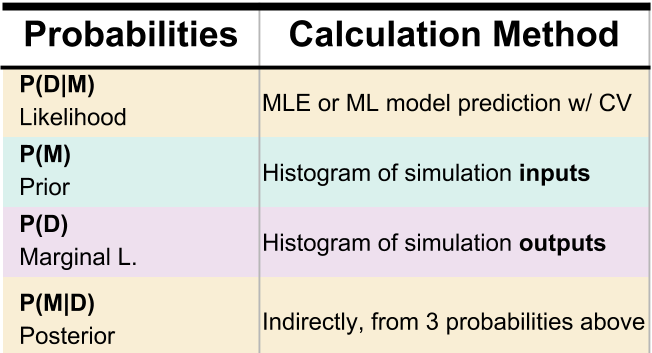
\includegraphics[width=\linewidth]{./figures/bayes-ch4.png}
      \caption{The density functions that represent each probability are estimated from histograms or the ML model}
    \end{table}
    \footnotesize
    Note: This implies the posterior is now only dependent on the likelihood.
  \end{minipage}
\end{frame}

\begin{frame}
  \frametitle{Posterior Odds}
  \textbf{Posterior odds $=$ probability of ML model $i$ being correct}
  \vfill
  \begin{enumerate}
    \item Calculate $MLE_i = P_i (m|d)$ for statistical model $i$
    \item Calculate $MLE_j = P_j (m|d)$ for statistical model $j$
    \item Ratio of $MLE_i$ to $MLE_j$ to get Bayes' factor:
          $B_{ij} = \frac{P_i (d|m)}{P_j (d|m)}$
    \item Take ratio of both Bayes' relations to get posterior odds:
          $\frac{P_i (m|d)}{P_j (m|d)} = B_{ij} \frac{P_i(m)}{P_j (m)}$
  \end{enumerate}
  \begin{table}
    \centering
    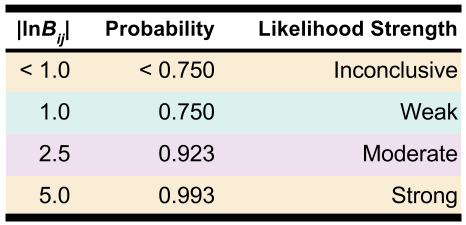
\includegraphics[width=0.6\linewidth]{./figures/evidence-strength.png}
    \caption{Model comparison using the Bayes' factor to describe the likelihood strength \cite{gentle_bayes, bayes_compare}}
  \end{table}
\end{frame}
